\section{Laplace Equation}
In order to use spherical harmonics to represent a surface, the gravitational potential at a point inside the body  must satisfy Poisson's Equation:
\begin{equation}
 \Delta V = -4\pi G \sigma
\end{equation}
  Inside the body has a density greater than zero. For a point outside the body, Laplace's equation (below) must be satisfied ( here there is no density outside the body):
\begin{equation} 
    \Delta V \equiv 0 
\end{equation}
 

\section{Spherical Harmonics}
Functions that satisfy Laplace's Equation are known as harmonic functions. Using a spherical coordinate system, spherical harmonic functions can then be used to represent the Earth's gravity field.
A Legendre function $ P_{nm}(cos\theta) $ is often used to calculate the geoid. The sign changes in any $ Y_{nm}(\theta,\lambda) $ in both directions divide the Earth into a chequer board pattern of  $(n-m+1) \times 2m  $ tiles as seen in the figure below \citep{nicoPhysicalgeodesy}:
\begin{figure}[h]
	\centering
	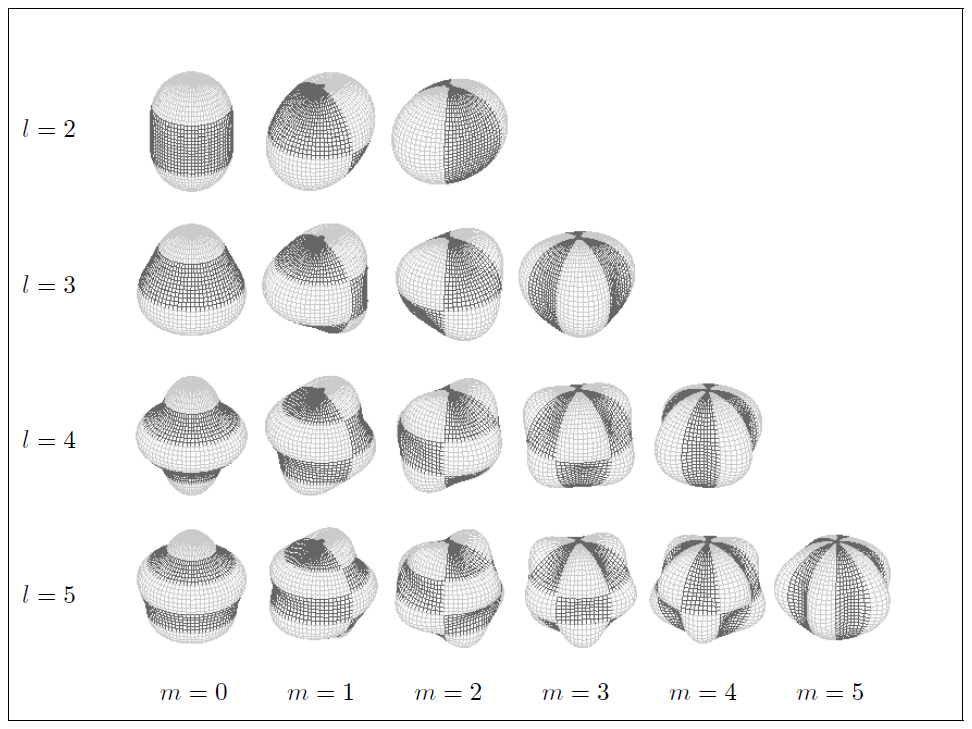
\includegraphics[width=0.5\textwidth]{earth.png}
	\caption{Spherical Harmonics up to Degree (l) and order (m) 5}
	\protect\citet{nicoPhysicalgeodesy}
	\label{fig:nicoearth}
\end{figure} 